%--------------------------------------------------------------------------
% !TEX root = 5Blman.tex
% dc1.tex
% 2013.01.06 changed to 2col format
%--------------------------------------------------------------------------
\chapter {DC Circuits Part I}

%---------------------------------------------------------------------
\begin{multicols}{2}
\section{Purpose}  
The purpose of this laboratory exercise is to explore series and parallel connections of resistances as well as series and parallel connections of emfs.  More importantly, you will practice the measurement and calculation of voltage, current, resistance, and power in simple circuits.

%---------------------------------------------------------------------
\section{Preparation}  
Read the material in your textbook regarding resistance, voltage, current, and simple DC circuits before coming to lab. Pay special attention to the major features of resistors in series and parallel and to the associated problem-solving strategies for them.

%---------------------------------------------------------------------
\section {Short quiz}  Be prepared to take a short quiz at the beginning of lab related to the concepts of series and parallel connections of resistors and emfs.

%---------------------------------------------------------------------
\section{General Information}
You will use three different methods to find resistance.  In the first you will simply use a color code to ``read'' the resistance value from the resistor markings. In the second method, you will the use an ohmmeter (one of the functions provided by a multimeter) to measure resistance directly.  In the third method you will use instruments to measure voltage across and current through a resistor, then calculate the resistance using Ohm's law --- this process is  referred to as ohm's method.

\begin{equation} R = V/I \label{e:ohm} \end{equation}

% \paragraph {You will calculate and measure the resistance of series and parallel connections of resistors.}  

Within experimental uncertainties the ohmmeter readings and the ohm's law measurements should be consistent.  Your instructor will inform you what error analysis to perform and direct you regarding how to report your results.

In series the total or equivalent resistance $R_S$ is 

\begin{equation} \label{e:ser}
	R_S  =  R_1  +  R_2  +  R_3  + \cdots	
\end{equation}

For resistors in parallel, the total or equivalent resistance $R_P$ is

\begin{equation} \label{e:par}
	%1/R_P  =  1/R_1  +  1/R_2  +  1/R_3  + \cdots
	R_P  =  \left (1/R_1  +  1/R_2  +  1/R_3  + \cdots \right)\relax^{-1}
\end{equation}

\paragraph {Some resistors are marked with colored bands to indicate the resistance they had at the time of manufacture.}  Although reading the color code does not constitute a measurement of resistance which may have changed over time by usage, it is useful to see what the nominal resistance should be.  The first and second colored bands give the first and second digits of the resistance.  The third band gives the power of ten and the fourth band indicates the precision of the manufactured resistance:  5\% for gold and  10\% for silver.

For example, if the bands are red, blue, green, and silver, the resistance is $26 \times 10^5$ with 10\% precision.

%\begin{table}
%\caption{Resistor Color Code}
%\centering
%\begin{tabular}{l c l c}Color & \# & Color & \# \\
%\hline
%Black	&	0 &	Green	& 5\\
%Brown	&	1 &	Blue	& 6\\
%Red		&	2 &	Violet	& 7\\
%Orange	&	3 &	Gray	& 8\\
%Yellow	&	4 &	White	& 9\\
%\end{tabular}
%\end{table}
%
%\begin{center}
%%\begin{tabularx}{\linewidth}{>{$}X<{$}>{$}X<{$}>{$}X<{$}}
%\begin{tabularx}{\linewidth}{XcXc}Color & \# & Color & \#}
%	\hline
%	Black	&	0 &	Green	& 5\\
%	Brown	&	1 &	Blue	& 6\\
%	Red		&	2 &	Violet	& 7\\
%	Orange	&	3 &	Gray	& 8\\
%	Yellow	&	4 &	White	& 9\\
%\end{tabularx}
%\mtcaption{Electric field values}
%\end{center}

\begin{center}
\begin{tabularx}{\linewidth}{@{}XXXc@{}}
	\hline
	Color	& \# & Color	& \# \\
	\hline
	Black	&	0 &	Green	& 5\\
	Brown	&	1 &	Blue	& 6\\
	Red		&	2 &	Violet	& 7\\
	Orange	&	3 &	Gray	& 8\\
	Yellow	&	4 &	White	& 9\\
\end{tabularx}
\mtcaption{Resistor Color Code}
\end{center}

\paragraph{Warning}  Your instructor will describe the operation of the instruments -- electronic multimeter, voltmeter, and ammeter.  Ammeters are instruments used to measure current and are particularly vulnerable to damage.  Have your instructor check your connections the first time you measure current to be certain that the meter is arranged correctly so that it is not damaged. The multimeter has a very low resistance when measuring current --  this allows the meter to be placed in series and not significantly change the resistance of the circuit.  The ammeter is placed in series so that it has the full current of the circuit branch passing through it.  This also makes the ammeter vulnerable to high currents and subsequent damage if it is connected directly to a voltage source.

%---------------------------------------------------------------------
\section {Measuring resistance}
These activities center on measuring resistance using three different methods. (1) Read the color code to get the value of a resistor. (2) Measure the resistor with an ohmmeter to get  its resistance value. (3) Measure voltage across and current through a resistor, then calculate the resistance value --- this process is  referred to as ohm's method.

%\begin{figure}[htb]
%	\centering
%	\includegraphics[scale=0.6]{5bgraf/mohm} %{5bgraf/fig_3}
%	\caption{Single resistor connected to an ohmmeter}
%	\label{f:mohm}
%\end{figure}

\begin{center}
	\includegraphics[scale=0.6]{5bgraf/mohm} %{5bgraf/fig_3}
	\mfcaption{Single resistor connected to an ohmmeter}
	\label{f:mohm}
\end{center}

\subsection{Activity: Ohm's law} \label{s:ohmlaw}
\begin{enumerate}
	\item \label{l:mm} Determine the individual resistances of three different resistors using the multimeter as indicated in \reffig{f:mohm}.
	
	\item \label{l:olm}Determine the resistances by the Ohm's law method in which applied voltage and current are measured and the resistance is calculated using  (\refeqn{e:ohm}).  The schematic in \reffig{f:mamblock} indicates how to set up these measurements.

	\item Make a table of the voltages and currents measured in item \ref{l:olm} and the resistances calculated from them.  Also list the measured values of resistance found directly with the multimeter from item \ref{l:mm} and those determined from the color code so that you can make side-by-side comparisons.

	\item Estimate the percent uncertainties in the voltage and current measurements and calculate the percent uncertainty in the resistances found in item \ref{l:olm} with the Ohm's law method.  Do the resistances found by the three different methods for each resistor agree with one another within these experimental uncertainties? If not, discuss why they might disagree.
	
	%\item Find the percent difference between the values of resistance found in item \ref{l:olm} and measurement by ohm's law and color code values. Discuss whether the values agree within experimental uncertainties.  If not, discuss why they might disagree.
	% This section can be confusing to read. Essentially, students are checking how direct measurement with an ohmmeter compares with current and voltage measurement followed by a calculation of resistance. This can also be compared with a direct rendering from the color code.
\end{enumerate}

%\begin{figure}[htb]
%	\centering
%	\includegraphics[scale=0.8]{5bgraf/mamblock} %{5bgraf/fig_4}
%	\caption{Measurement of current through and voltage across a resistor}
%	\label{f:mamblock} %{f:fig4}
%\end{figure}

\begin{center}
	\includegraphics[scale=0.8]{5bgraf/mamblock} %{5bgraf/fig_4}
	\mfcaption{Measurement of current through and voltage across a resistor}
	\label{f:mamblock} %{f:fig4}
\end{center}

\subsection{Activity: Resistances in series} \label{s:series}
\begin{enumerate}
	\item \label{l:eqs} Determine the equivalent resistance of each resistor connected in series using the Ohm's law method. To do this measure the voltage across each resistor separately and the current through it. The current is the same through each resistor. The schematic in \reffig{f:mamblock} shows the measurement of the voltage across and the current through a single resistor. Use  \reffig{f:fig5}. to measure the voltages and current for multiple resistors in series.
	
	\item Once you have measured the voltage and current for each resistor separately, calculate the equivalent series resistance $R_S$ using equation \ref{e:ohm}.
	
	\item Determine the experimental uncertainty in the value of $R_S$. %found in item \ref{l:eqs}.
	
	\item Calculate the equivalent resistance $R_S$ using equation (\ref{e:ser}) where the individual resistances are those found by the Ohm's law method. %in item \ref{l:olm}.
\end{enumerate}

%\begin{figure}
%	\centering
%	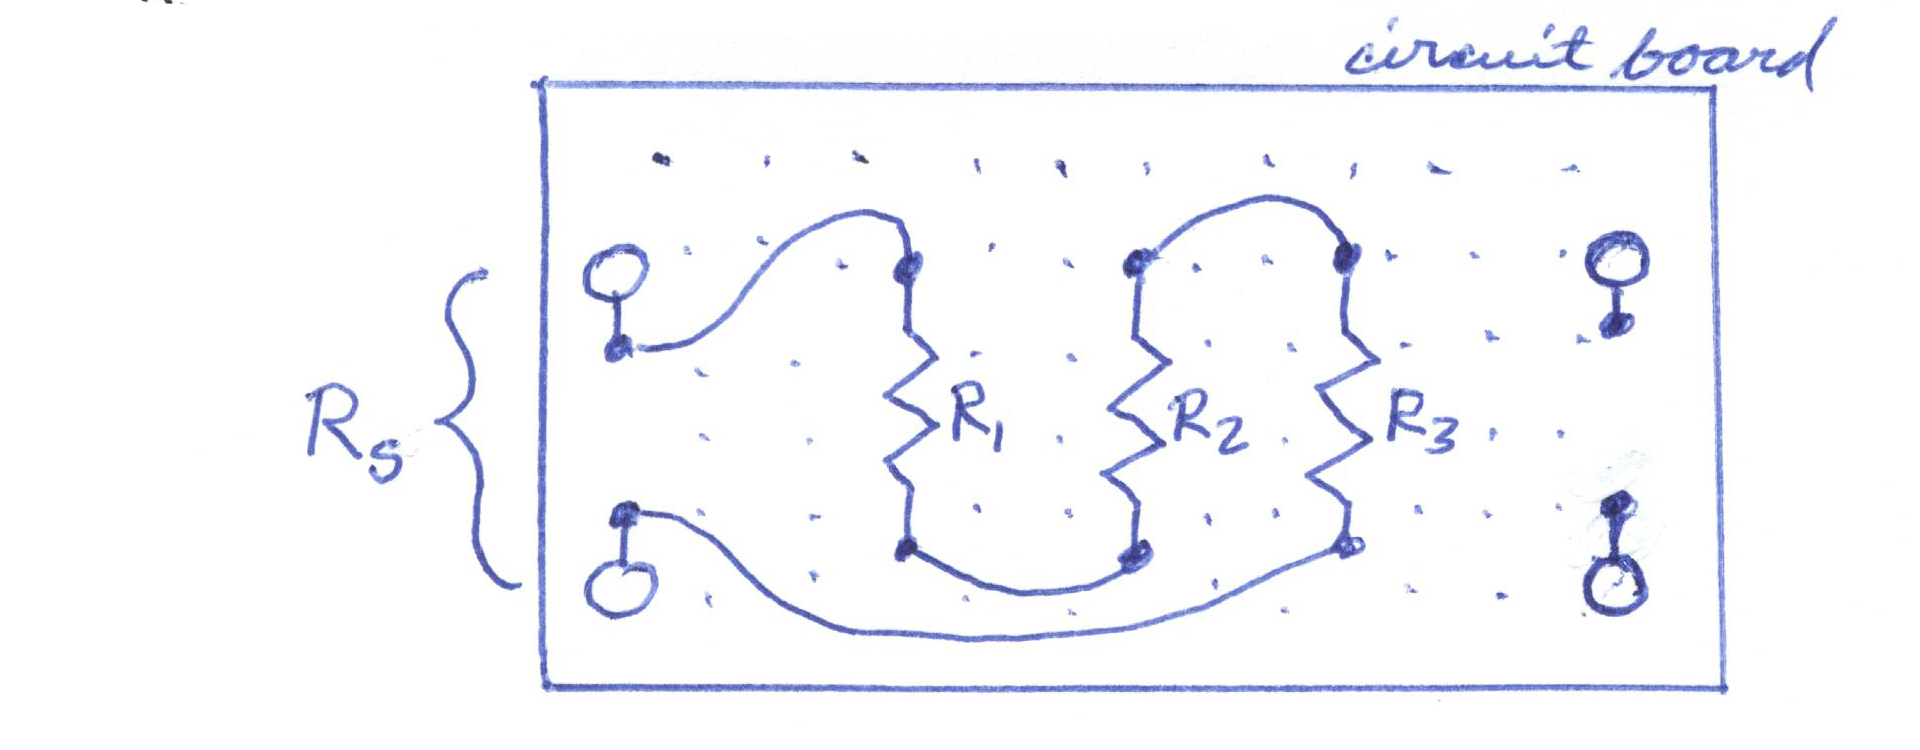
\includegraphics[scale=0.8]{5bgraf/fig_5}
%	\caption{Resistors in series}
%	\label{f:fig5}
%\end{figure}

%\begin{figure}[htb] \centering
% \subfloat[series circuit]
%   {\includegraphics[scale=0.5]{5bgraf/r3series}\label{f:fig5}} % fig_5
% \hfill
% \subfloat[parallel circuit]
%   {\includegraphics[scale=0.5]{5bgraf/r3parallel}\label{f:fig6}} % fig_6
% \caption{Resistors in series and parallel}\label{f:serpar}
%\end{figure}

\begin{center}
   {\includegraphics[scale=0.5]{5bgraf/r3series}
   \label{f:fig5}} % fig_5
% \hfill
   {\includegraphics[scale=0.5]{5bgraf/r3parallel}
   \label{f:fig6}} % fig_6
 \mfcaption{Resistors in series and parallel}
 \label{f:serpar}
\end{center}


\subsection{Activity: Resistances in parallel}
\begin{enumerate}
	\item Determine the equivalent resistance of three resistors connected in parallel using the Ohm's law method.  Again, review \reffig{f:mamblock} to remind yourself how to measure voltage and current for a single resistor --- use fig. \reffig{f:fig6} for voltage and current measurements of multiple resistors in parallel.
	
	\item Calculate the equivalent resistance $R_P$ using equation (\ref{e:ohm}) where the individual resistances are those found by the Ohm's law method.

	\item Once you have measured the voltage and current, calculate the equivalent parallel resistance $R_P$ using equation (\ref{e:par}).
	
	\item Determine the experimental uncertainty in the value of $R_P$.
\end{enumerate}

%\begin{figure}
%	\centering
%	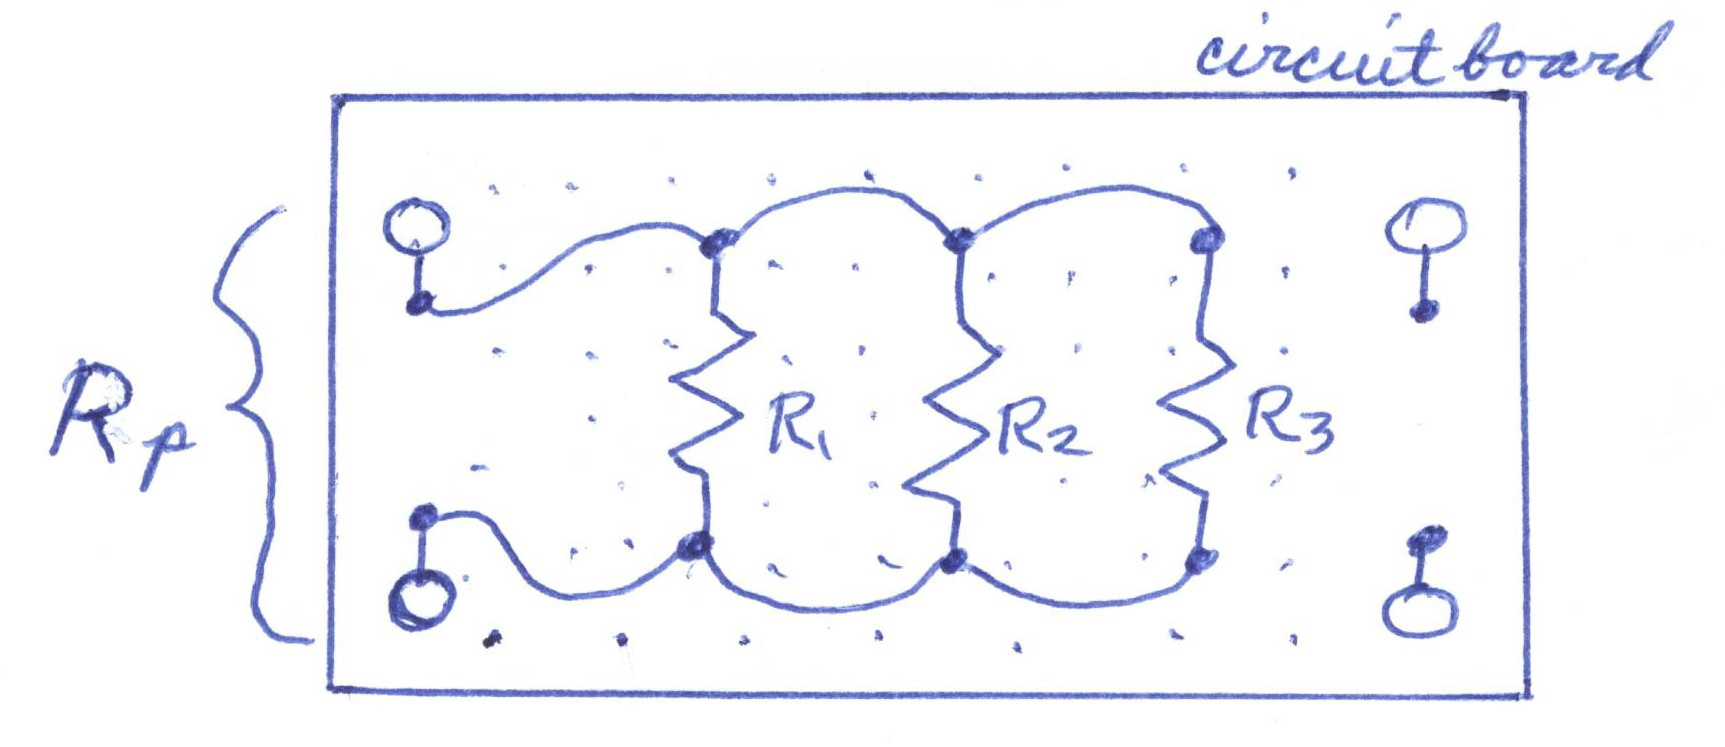
\includegraphics[scale=0.8]{5bgraf/fig_6}
%	\caption{Resistors in parallel}
%	\label{f:fig6}
%\end{figure}

\subsection{Activity: EMF's in series and parallel}
\begin{enumerate}
	\item Measure the emfs of two individual dry cells and the total emfs when they are placed in series and in parallel as shown in \reffig{f:vseriespar}.
	
	\item Explain the values obtained in the series and parallel connections.
	
	\item Do they agree with theory?  If not, could the internal resistance of the emfs be responsible for the disagreement or is it within experimental uncertainties?
\end{enumerate}

%\begin{figure}[htbp]
%	\centering
%	\includegraphics[scale=0.7]{5bgraf/mvoltswitch}
%	\caption{Measurement of single dry cell}
%	\label{f:mvoltswitch}
%\end{figure}
%
%
%\begin{figure}[htb]
%	\centering
%	\includegraphics[scale=.9]{5bgraf/vseriespar} %{5bgraf/fig_7}
%	\mfcaption{Battery configurations in series and parallel}
%	\label{f:vseriespar} %{f:fig7}
%\end{figure}

\begin{center}
	\includegraphics[scale=0.7]{5bgraf/mvoltswitch}
	\mfcaption{Measurement of single dry cell}
	\label{f:mvoltswitch}
\end{center}

\begin{center}
	\includegraphics[scale=.9]{5bgraf/vseriespar} %{5bgraf/fig_7}
	\mfcaption{Battery configurations in series and parallel}
	\label{f:vseriespar} %{f:fig7}
\end{center}


\paragraph{If time permits}  Using the set-up in \reffig{f:fig5}, measure the voltage drops across each of the three resistors and compare these with the terminal voltage of the dry cell.  Discuss the meaning of your results.

\end{multicols}


%\clearpage
%%\newpage
%\includegraphics*[width=\textwidth,trim=120 80 80 120,clip]{5bgraf/pslabgrid} 

%--------------------------------------------------------------------------
\endinput
%--------------------------------------------------------------------------
